% ============================================================
% Stage detector positioning in the defense pipeline
% Compile with:  pdflatex stage_detector_position.tex
% Output:        stage_detector_position.pdf
% ============================================================
\documentclass[border=4pt]{standalone}
\usepackage{tikz}
\usetikzlibrary{shapes.geometric, arrows.meta, positioning, fit, backgrounds, calc}

\definecolor{colFeat}{RGB}{220,235,245}
\definecolor{colDet}{RGB}{245,235,215}
\definecolor{colRL}{RGB}{220,245,220}
\definecolor{colBorder}{RGB}{80,100,120}
\definecolor{colArrow}{RGB}{60,80,100}

\tikzset{
  box/.style={
    rectangle, rounded corners=3pt,
    draw=colBorder, line width=0.7pt,
    text centered, font=\small,
    inner sep=5pt, minimum height=1.8em
  },
  featBox/.style={box, fill=colFeat, minimum width=2.8cm, minimum height=1.6cm, align=center},
  detBox/.style={box, fill=colDet, minimum width=3.0cm, minimum height=1.6cm, align=center},
  rlBox/.style={box, fill=colRL, minimum width=3.0cm, minimum height=1.6cm, align=center},
  arr/.style={
    -{Stealth[length=5pt]}, line width=0.8pt, color=colArrow
  },
  label/.style={font=\footnotesize, text=colBorder}
}

\begin{document}
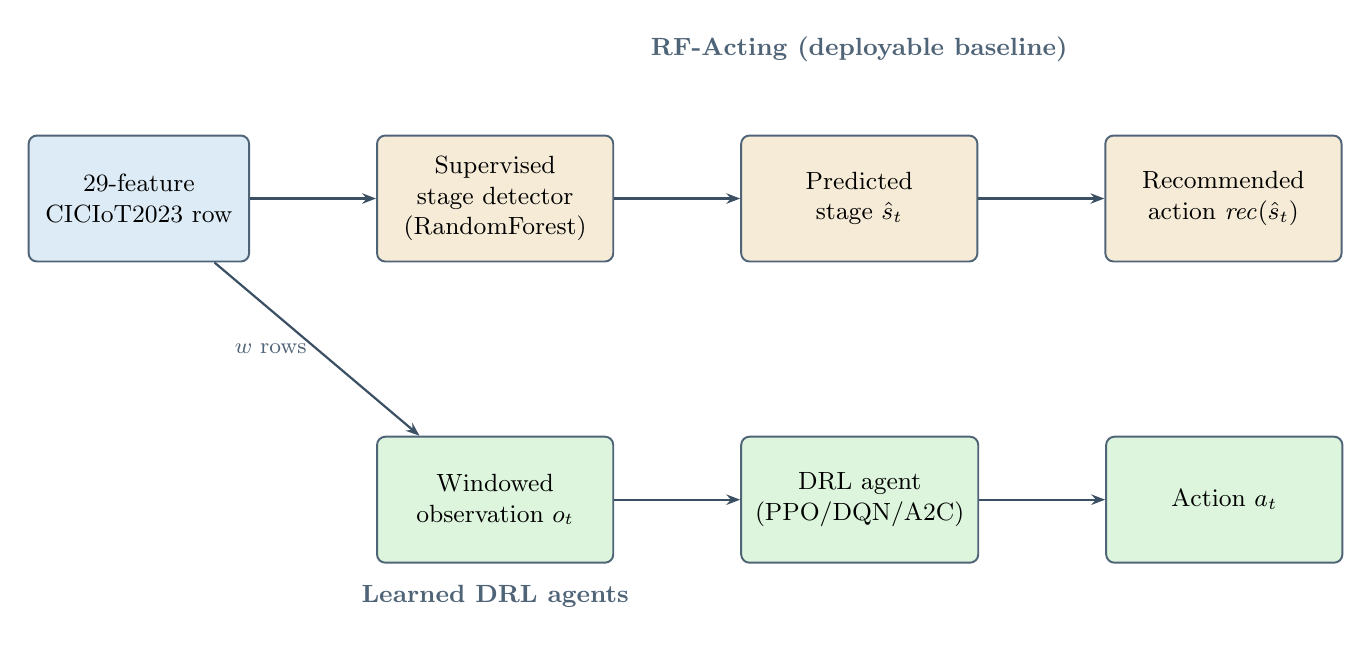
\begin{tikzpicture}[node distance=1.6cm]

  \node[featBox] (feat) {29-feature\\CICIoT2023 row};

  \node[detBox, right=of feat] (det) {Supervised\\stage detector\\(RandomForest)};
  \node[detBox, right=of det] (stage) {Predicted\\stage $\hat{s}_t$};
  \node[detBox, right=of stage] (rec) {Recommended\\action $\mathit{rec}(\hat{s}_t)$};

  \node[rlBox, below=2.2cm of det] (window) {Windowed\\observation $o_t$};
  \node[rlBox, right=of window] (rl) {DRL agent\\(PPO/DQN/A2C)};
  \node[rlBox, right=of rl] (action) {Action $a_t$};

  % RF-Acting path
  \draw[arr] (feat) -- node[label, above] {} (det);
  \draw[arr] (det) -- node[label, above] {} (stage);
  \draw[arr] (stage) -- node[label, above] {} (rec);

  % RL path
  \draw[arr] (feat) -- node[label, left] {$w$ rows} (window);
  \draw[arr] (window) -- (rl);
  \draw[arr] (rl) -- (action);

  % contrast label
  \node[font=\small\bfseries, text=colBorder, above=0.8cm of stage] {RF-Acting (deployable baseline)};
  \node[font=\small\bfseries, text=colBorder, below=0.15cm of window] {Learned DRL agents};

\end{tikzpicture}
\end{document}
